\chapter{BÀI TOÁN PHÁT HIỆN TIN NÓNG VÀ CÁC PHƯƠNG PHÁP TIẾP CẬN PHỔ BIẾN}
\ifpdf
    \graphicspath{{Chapter2/Chapter2Figs/PNG/}{Chapter2/Chapter2Figs/PDF/}{Chapter2/Chapter2Figs/}}
\else
    \graphicspath{{Chapter2/Chapter2Figs/EPS/}{Chapter2/Chapter2Figs/}}
\fi

\section{Mở đầu}
Chương này sẽ giới thiệu bài toán phát hiện và theo dõi tin tức. Trình bày cơ sở lý thuyết và phát biểu bài toán phát hiện tin nóng. Cuối cùng trình bày một số phương pháp tiếp cận bài toán phát hiện tin nóng và các kiến thức liên quan.
\section{Giới thiệu bài toán} %Topic Detection and Tracking}
	\subsection{Các khái niệm cơ bản}
	Để có thể xác định khái niệm tin nóng, trước hết ta cần xem xét định nghĩa của "sự kiện" và "mẩu tin". Fiscus và Doddington \cite{Fiscus:TDTDefinition} đã tóm tắt định nghĩa về event và story như sau:
	\begin{itemize}
		\item \textit{Sự kiện (event)} là một sự việc bất kì, xảy ra tại một địa điểm cụ thể vào thời điểm xác định, cùng với những điều kiện dẫn đến nó và các hậu quả kéo theo.
		
		\item \textit{Mẩu tin (story)} là một bài viết liên quan đến một chủ đề nhất định. Có ít nhất 2 câu trần thuật độc lập với nhau.
	\end{itemize}
	
	Dựa trên quan điểm trên, ta định nghĩa tin nóng như sau:
	
	\textbf{Định nghĩa:} Tin nóng là những tin viết về một sự kiện mới xảy ra, có tính thời sự, có tầm ảnh hưởng rộng, thu hút được sự chú ý, quan tâm của cộng đồng.

%
	\subsection{Bài toán Topic Detection and Tracking}
	Topic Detection and Tracking (TDT) là một dự án bao quát được khởi xướng từ năm 1996, với mục tiêu nghiên cứu, phát triển công nghệ cho việc lưu trữ, tổ chức, tìm kiếm dữ liệu từ các nguồn \textit{tin tức} \cite{Fiscus:TDTDefinition}.
	
	Nhiệm vụ của TDT là xử lý luồng dữ liệu văn bản liên tục (từ báo chí, từ đài phát thanh, đài truyền hình thông qua các bộ chuyển giọng nói thành văn bản), từ đó theo dõi và phát hiện được các sự kiện đang diễn ra, cũng như tổ chức các bài viết thành những nhóm cùng bàn về một sự kiện nào đó.
	
	Theo Fiscus và Doddington \cite{Fiscus:TDTDefinition}, TDT được chia làm 5 tác vụ chính: 
		\begin{itemize}
			\item Story segmentation: phân đoạn dữ liệu từ đài phát thanh thành những mẩu tin riêng biệt.
			\item Topic detection: Gom nhóm các bài viết theo sự kiện, chủ đề chúng đề cập tới.
			\item Topic tracking: Theo dõi những chuyển biến của sự kiện đã diễn ra.
			\item First story detection: Phát hiện tin tức đầu tiên nói về sự kiện vừa xảy ra.
			\item Link detection: Xác định xem một cặp bài viết ngẫu nhiên có đang đề cập về cùng sự kiện không.
		\end{itemize}

	\subsection{Bài toán phát hiện tin nóng}
	Bài toán phát hiện tin nóng có thể xem là sự kết hợp giữa hai bài toán Topic Detection và First Story Detection (FSD) của TDT. Theo James Allan \cite{Allan:2002:ITD:772260.772262}, bài toán First Story Detection, hay còn gọi là New Event Detection, được đặt ra với mục tiêu phát hiện các tin tức, bài viết đầu tiên trên báo chí về các sự kiện vừa xảy ra, chưa từng được báo cáo trước đó. Ví dụ như bài viết đầu tiên đưa thông tin về một vụ tai nạn, khủng bố, hay một vụ scandal chính trị nào đó. Một hệ thống có khả năng phát hiện các first story có thể cung cấp thông tin hữu ích cho các nhà phân tích, các biên tập viên báo chí một cách nhanh chóng, kịp thời.
	
	Đối với bài toán Topic Detection, nhiệm vụ chính là gom các bài viết về cùng một sự kiện thành từng cụm, mỗi cụm là đại diện cho một sự kiện cụ thể nào đó. Do tính chất của bài toán, ta không được biết trước số lượng sự kiện (số cụm) hay nội dung từng sự kiện như thế nào, điều này hoàn toàn bởi hệ thống tự động xác định. So với FSD, bài toán này tập trung nhiều hơn vào việc nhóm được phần lớn các bài viết liên quan lại với nhau, hơn là việc phát hiện bài viết đầu tiên. Tuy nhiên trên thực tế, nhiều nhà nghiên cứu sử dụng chung một hướng giải quyết cho cả 2 bài toán này \cite{Allan:2002:ITD:772260.772262}.
	
	Ngoài nguồn dữ liệu từ báo đài, các bài viết từ mạng xã hội cũng là một nguồn tin có tiềm năng khai thác rất lớn. Tuy chất lượng bài viết và tính xác thực về nội dung có thể không tốt bằng các nguồn chính thống, các tin tức từ mạng xã hội thường có lợi thế về mặt tốc độ đưa tin. Một ví dụ nổi bật cho tính chất này là sự kiện Osama Bin Laden bị ám sát vào năm 2011, khi đó một người dùng là Keith Urbahn đã đưa thông tin lên Twitter nhanh hơn giới truyền thông đến 21 phút.

	\subsection{Phát biểu bài toán phát hiện tin nóng từ Twitter}
	Cho trước $D = (d_1, d_2, d_3,... d_n)$: chuỗi các bài viết từ Twitter được sắp xếp theo thứ tự thời gian.
	
	Mục tiêu của bài toán là phát hiện được các cụm tin $C = (c_1, c_2,... c_m)$, với mỗi phần tử $c_i = (d_{i1}, d_{i2},... d_{ik})$ là chuỗi các bài viết bàn về cùng một sự kiện cụ thể, và $d_{i1}$ là bài viết đầu tiên viết về sự kiện đó. Danh sách các chuỗi tin $C$  được sắp xếp theo thứ tự độ nóng giảm dần, với độ nóng được tính toán dựa trên thời gian đăng tin, tầm ảnh hưởng và mức độ quan tâm cộng đồng đối với sự kiện được đề cập.
	
%	Input: Tập bài viết theo thứ tự thời gian $D = \{d_1, d_2, d_3,... d_n\}$ từ nguồn Twitter.
%	Output: Tập cụm bài viết $C = \{c_1, c_2, c_3,... c_k\}$, có sắp xếp thứ tự độ quan trọng, mỗi cụm đại diện cho một sự kiện vừa diễn ra, và bài viết đầu tiên trong cụm là first story.
	
%\section{Biểu diễn dữ liệu bằng Vector space model và tf-idf}
\section{Thuật toán Naive Bayes}
\subsection{Giới thiệu thuật toán Naive Bayes}
	 Thuật toán Naive Bayes là một thuật toán phân lớp xác suất đơn giản dùng để tính một tập các xác suất bằng cách đếm tần suất và kết hợp của các giá trị trong một tập cho trước. Thuật toán sử dụng định luật Bayes sẽ giả định rằng tất cả các chiều(attributes) của dữ liệu là độc lập với nhau. Các giả định rằng các chiều là độc lập với nhau rất khó để có thể xuất hiện trong thực tế. Tuy nhiên giả thiết ngây ngô này lại mang lại những kết quả phân lớp tốt cho nhiều bài toán phân lớp \cite{dimitoglou2012comparison}.
\subsection{Lý thuyết Bayes}
    Định lý Bayes cho phép tính xác suất xảy ra của một sự kiện ngẫu nhiên A khi biết sự kiện liên quan B đã xảy ra. Xác suất này được ký hiệu là P(A|B), và đọc là “xác suất của A nếu có B”. Đại lượng này được gọi xác suất có điều kiện hay xác suất hậu nghiệm vì nó được rút ra từ giá trị được cho của B hoặc phụ thuộc vào giá trị đó.

	Theo định lí Bayes, xác suất xảy ra A khi biết B sẽ phụ thuộc vào 3 yếu tố:
	
	Xác suất xảy ra A của riêng nó, không quan tâm đến B. Kí hiệu là P(A) và đọc là xác suất của A. Đây được gọi là xác suất biên duyên hay xác suất tiên nghiệm, nó là “tiên nghiệm” theo nghĩa rằng nó không quan tâm đến bất kỳ thông tin nào về B.
	
	Xác suất xảy ra B của riêng nó, không quan tâm đến A. Kí hiệu là P(B) và đọc là “xác suất của B”. Đại lượng này còn gọi là hằng số chuẩn hóa (normalising constant), vì nó luôn giống nhau, không phụ thuộc vào sự kiện A đang muốn biết.
	
	Xác suất xảy ra B khi biết A xảy ra. Kí hiệu là P(B|A) và đọc là “xác suất của B nếu có A”. Đại lượng này gọi là khả năng (likelihood) xảy ra B khi biết A đã xảy ra. Chú ý không nhầm lẫn giữa khả năng xảy ra B khi biết A và xác suất xảy ra A khi biết B.
	
	Tóm lại định lý Bayes sẽ giúp ta tính ra xác suất xảy ra của một giả thuyết bằng cách thu thập các bằng chứng nhất quán hoặc không nhất quán với một giả thuyết nào đó. Khi các bằng chứng tích lũy, mức độ tin tưởng vào một giả thuyết thay đổi. Khi có đủ bằng chứng, mức độ tin tưởng này thường trở nên rất cao hoặc rất thấp, tức là xác xuất sảy ra giả thuyết sẽ thay đổi thì các bằng chứng liên quan đến nó thay đổi.
	
	Công thức của định luật Bayes được phát biểu như sau:
\begin{equation}
	P(A \mid B) = \frac{P(B \mid A) \, P(A)}{P(B)}
\end{equation}
Trong đó:
\begin{itemize}
	\item P(A|B) là  xác suất xảy ra của một sự kiện ngẫu nhiên A khi biết sự kiện liên quan B đã xảy ra.
	\item P(B|A) là xác suất xảy ra B khi biết A xảy ra
	\item P(A) là xác suất sảy ra của riêng A mà không quan tâm đến B.
	\item P(B) là xác suất xảy ra của riêng B mà không quan tâm đến A.
\end{itemize}
	Ở trên ta có thể thấy xác suất sảy ra của giả thuyết A phụ thuộc và xác suất của giả thuyết B, nhưng trong thực tế xác suất A có thể phụ thuộc vào xác suất của nhiều các giác thuyết khác có thể là B1, B2, B3 … Bn. Vậy định luật Bayes có thể được mở rộng bằng công thức sau:
\begin{equation}
	P(A \mid B) = \frac{\left(P(B_1 \mid A) \times P(B_2 \mid A) \times P(B_3 \mid A)... \times P(B_n \mid A)\right) \times P(A)}{P(B_1) \times P(B_2) \times P(B_3)... \times P(B_n)}
\end{equation}
\subsection{Naive Bayes Classifier}
	Xét bài toán classification với C classes 1,2,…,C. Giả sử có một điểm dữ liệu $x \in \mathbb{R}^d $. Hãy tính xác suất để điểm dữ liệu này rơi vào class c. Nói cách khác, hãy tính:
\begin{equation}
	p(y = c \mid x)
\end{equation}
	hoặc viết gọn là $p(c \mid x)$
	Tức tính xác suất để đầu ra là class c biết rằng đầu vào là vector x.
	Biểu thức này, nếu tính được, sẽ giúp chúng ta xác định được xác suất để điểm dữ liệu rơi vào mỗi class. Từ đó có thể giúp xác định class của điểm dữ liệu đó bằng cách chọn ra class có xác suất cao nhất:
\begin{equation}
	c = \arg\max_{c \in \left\{1,..,C \right\}} p(c \mid x)
\end{equation}
Biểu thức (2) thường khó được tính trực tiếp. Thay vào đó, quy tắc Bayes thường được sử dụng:
\begin{align}
	c = \arg\max_{c } p(c \mid x) \label{NB1} \\
	  = \arg\max_{c }\frac{p(x \mid c) p(c)}{p(x)} \label{NB2} \\
	  = \arg\max_{c } p(x \mid c) p(c) \label{NB3}
\end{align}
	Từ \eqref{NB1} sang \eqref{NB2} là vì quy tắc Bayes. Từ \eqref{NB2} sang \eqref{NB3} là vì mẫu số p(x) không phụ thuộc vào c.
	Tiếp tục xét biểu thức \eqref{NB3}, p(c) có thể được hiểu là xác suất để một điểm rơi vào class c. Giá trị này có thể được tính bằng MLE, tức tỉ lệ số điểm dữ liệu trong tập training rơi vào class này chia cho tổng số lượng dữ liệu trong tập traing; hoặc cũng có thể được đánh giá bằng MAP estimation. Trường hợp thứ nhất thường được sử dụng nhiều hơn.
	
	Thành phần còn lại p(x|c), tức phân phối của các điểm dữ liệu trong class c, thường rất khó tính toán vì x là một biến ngẫu nhiên nhiều chiều, cần rất rất nhiều dữ liệu training để có thể xây dựng được phân phối đó. Để giúp cho việc tính toán được đơn giản, người ta thường giả sử một cách đơn giản nhất rằng các thành phần của biến ngẫu nhiên x là độc lập với nhau, nếu biết c (given c..) Tức là:
\begin{equation}
	p(x \mid c) = p(x_1,x_2,...,x_d \mid c) = \displaystyle \prod_{i=1}^d p(x_i \mid c)
\end{equation}
	Khi một dữ liệu mới được thêm vào, Naive Bayes sẽ xác định lớp của điểm dữ liệu x bởi:
\begin{equation}
	c = \arg\max_{c \in \left\{ 1,...,C\right\}} p(c) \prod_{i=1}^{d}p(x_i \mid c) 
	\label{NB4}
\end{equation}
Khi d lớn và các xác suất nhỏ, biểu thức ở vế phải của \ref{NB4} sẽ là một số rất nhỏ, khi tính toán có thể gặp sai số. Để giải quyết việc này, \ref{NB4} thường được viết lại dưới dạng tương đương bằng cách lấy log của vế phải:
 \begin{equation}
 	c = \arg\max_{c \in \left\{ 1,...,C\right\}} = \log(p(c) + \sum_{i=1}^{d}\log(p(x_i \mid c)))
 \end{equation}
	Việc này không ảnh hưởng tới kết quả vì log là một hàm đồng biến trên tập các số dương.
	 
	Mặc dù giả thiết mà Naive Bayes Classifiers sử dụng là quá phi thực tế, chúng vẫn hoạt động khá hiệu quả trong nhiều bài toán thực tế, đặc biệt là trong các bài toán phân loại văn bản, ví dụ như lọc tin nhắn rác hay lọc email spam. Trong phần sau của bài viết, chúng ta cùng xây dựng một bộ lọc email spam tiếng Anh đơn giản.
	 
	Cả việc training và test của NBC là cực kỳ nhanh khi so với các phương pháp classification phức tạp khác. Việc giả sử các thành phần trong dữ liệu là độc lập với nhau, nếu biết class, khiến cho việc tính toán mỗi phân phối p(xi|c) trở nên cực kỳ nhanh.
	 
	Mỗi giá trị p(c),c=1,2,…,C có thể được xác định như là tần suất xuất hiện của class c trong training data.
	 
	Việc tính toán p(xi|c) phụ thuộc vào loại dữ liệu. Có ba loại được sử dụng phổ biến là: Gaussian Naive Bayes, Multinomial Naive Bayes, và Bernoulli Naive.
\subsection{Một số phân phối thường dùng}
	\subsubsection{Gaussian Naive Bayes}
		Mô hình này được sử dụng chủ yếu trong loại dữ liệu mà các thành phần là các biến liên tục. Với mỗi chiều dữ liệu i và một class c, xi tuân theo một phân phối chuẩn có kỳ vọng $ \mu_{ci} $ và phương sai $\sigma_{ci}^2$:
	\begin{equation}
		p(x_i \mid c) = p(x_i \mid \mu_{ci}, \sigma_{ci}^2)=\frac{1}{\sqrt{2\pi\sigma_{ci}^2}}\exp(\frac{(x_i - \mu_{ci})^2}{2 \sigma_{ci}^2})  
	\end{equation}
		Trong đó, bộ tham số $\theta = { \mu_{ci}, \sigma_{ci}^2}$ được xác định bằng Maximum Likehood
	\begin{equation}
		(\mu_{ci}, \sigma_{ci}^2)=\arg\max_{\mu_{ci}, \sigma_{ci}^2}\prod_{i=1}^n p(x_i^(n) \mid \mu_{ci},\sigma_{ci}^2 )
	\end{equation}
	\subsubsection{Multinominal Naive Bayes}
	Mô hình này chủ yếu được sử dụng trong phân loại văn bản mà feature vectors được tính bằng Bags of Words. Lúc này, mỗi văn bản được biểu diễn bởi một vector có độ dài d chính là số từ trong từ điển. Giá trị của thành phần thứ i trong mỗi vector chính là số lần từ thứ i xuất hiện trong văn bản đó.
	
	Khi đó, p(xi|c) tỉ lệ với tần suất từ thứ i (hay feature thứ i cho trường hợp tổng quát) xuất hiện trong các văn bản của class c. Giá trị này có thể được tính bằng cách:
	\begin{equation}
		\lambda_{ci}=p(x_i \mid c) = \frac{N_ci}{N_c}
	\end{equation}
	Trong đó:
	\begin{itemize}
		\item $N_ci$ là tổng số lần từ thứ i xuất hiện trong các văn bản của class c, nó được tính là tổng của tất cả các thành phần thứ i của các feature vectors ứng với class c
		\item $N_c$ là tổng số từ (kể cả lặp) xuất hiện trong class c. Nói cách khác, nó bằng tổng độ dài của toàn bộ các văn bản thuộc vào class c. Có thể suy ra rằng $N_c$=$ \sum_{i=1}^d=N_ci$, từ đó =$ \sum_{i=1}^d \lambda_{ci}=1$.
	\end{itemize}
		
	Cách tính này có một hạn chế là nếu có một từ mới chưa bao giờ xuất hiện trong class c
	thì biểu thức (10) sẽ bằng 0, điều này dẫn đến vế phải của (7) bằng 0 bất kể các giá trị còn lại có lớn thế nào. Việc này sẽ dẫn đến kết quả không chính xác (xem thêm ví dụ ở mục sau).
	Để giải quyết việc này, một kỹ thuật được gọi là Laplace smoothing được áp dụng:
	\begin{equation}
		\hat{\lambda_{ci}} = \frac{N_{ci}+ \alpha}{N_c+d_\alpha}
	\end{equation}
	Với $\alpha$ là một số dương, thường bằng 1, để tránh trường hợp tử số bằng 0. Mẫu số được cộng với $d_\alpha$ để đảm bảo tổng xác suất $ \sum_{i=1}^d \hat{\lambda_{ci}}=1$.
	Như vậy, mỗi class c sẽ được mô tả bởi bộ các số dương có tổng bằng 1: $ \hat{\lambda_{c}}= \left\{\hat{\lambda_{c1}}+,...,+\hat{\lambda_{cd}}\right\}$.
	\subsubsection{Bernoulli Naive}
	Mô hình này được áp dụng cho các loại dữ liệu mà mỗi thành phần là một giá trị binary - bẳng 0 hoặc 1. Ví dụ: cũng với loại văn bản nhưng thay vì đếm tổng số lần xuất hiện của 1 từ trong văn bản, ta chỉ cần quan tâm từ đó có xuất hiện hay không.
	
	Khi đó, $p(x_i \mid c $ được tính bằng:
	\begin{equation}
		p(x_i \mid c) = p(i \mid c)x_i + 1-p(i\mid c)(1- x_i)
	\end{equation}
	với p(i|c) có thể được hiểu là xác suất từ thứ i xuất hiện trong các văn bản của class c.
	 
	\subsection{Ưu điểm thuật toán Naive Bayes}
	\subsection{Nhược điểm điểm thuật toán Naive Bayes}
	\subsection{Naive Bayes với bài toán lọc rác tin tức}
\section{Thuật toán J48}
	\subsection{Giới thiệu thuật toán J48}
		Thuật toán J48(C4.5) là một thuật toán sử dụng cây quyết định(decision tree) cho việc phân lớp. Thuật toán sẽ tạo ra môn cây nhị phân. Bằng cách sử dụng cây quyết định, cách tiếp cận này cũng thường đước sử dụng trong bài toán phân lớp. Cây quyết định sẽ được xây dựng để mô hình hóa quá trình phân lớp.
	\subsection{Lý thuyết cây quyết định}
		Cây quyết định (Decision Tree) là một cây phân cấp có cấu trúc được dùng để phân lớp các đối tượng dựa vào dãy các luật (series of rules). Các thuộc tính của đối tượng (ngoại trừ thuộc tính phân lớp – Category attribute) có thể thuộc các kiểu dữ liệu khác nhau (Binary, Nominal, ordinal, quantitative values) trong khi đó thuộc tính phân lớp phải có kiểu dữ liệu là Binary hoặc Ordinal.
		Tóm lại, cho dữ liệu về các đối tượng gồm các thuộc tính cùng với lớp (classes) của nó, cây quyết định sẽ sinh ra các luật để dự đoán lớp của các đối tượng chưa biết (unseen data)
	\subsection{Ví dụ về cây quyết định J48}
	\begin{figure}[H]
		\centering
		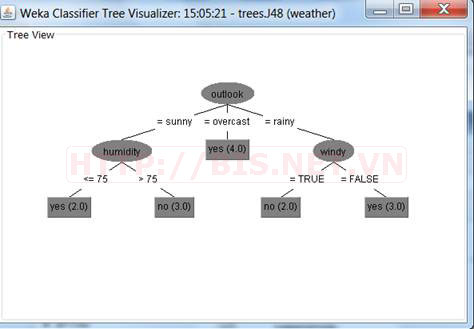
\includegraphics[width=0.9\linewidth]{Chapter2/Chapter2Figs/Decision_Tree_007}
		\caption{Ví dụ về cây quyết định}
		\label{fig:DecisionTreeExample}
	\end{figure}
\section{Tiền xử lý dữ liệu}
Giai đoạn tiền xử lý dữ liệu
Quá trình xử lý dữ liệu thô/gốc (raw/original data) nhằm cải thiện chất lượng dữ liệu (quality of the data) và do đó, cải thiện chất lượng của kết quả khai phá.
Dữ liệu thô/gốc
	Có cấu trúc, bán cấu trúc, phi cấu trúc
	Được đưa vào từ các nguồn dữ liệu trong các hệ thống xử lý tập tin (file processing systems) và/hay các hệ thống cơ sở dữ liệu (database systems)
Chất lượng dữ liệu (data quality): tính chính xác, tính hiện hành, tính toàn vẹn, tính nhất quán 
Chất lượng dữ liệu (data quality)
	tính chính xác (accuracy): giá trị được ghi nhận đúng với giá trị thực.
	tính hiện hành (currency/timeliness): giá trị được ghi nhận không bị lỗi thời.
	tính toàn vẹn (completeness): tất cả các giá trị dành cho một biến/thuộc tính đều được ghi nhận.
	tính nhất quán (consistency): tất cả giá trị dữ liệu đều được biểu diễn như nhau trong tất cả các trường hợp.
	
	Các kỹ thuật tiền xử lý dữ liệu
		Làm sạch dữ liệu (data cleaning/cleansing): loại bỏ nhiễu (remove noise), hiệu chỉnh những phần dữ liệu không nhất quán (correct data inconsistencies)
		Tích hợp dữ liệu (data integration): trộn dữ liệu (merge data) từ nhiều nguồn khác nhau vào một kho dữ liệu
		Biến đổi dữ liệu (data transformation): chuẩn hoá dữ liệu (data normalization)
		Thu giảm dữ liệu (data reduction): thu giảm kích thước dữ liệu (nghĩa là giảm số phần tử) bằng kết hợp dữ liệu (data 	aggregation), loại bỏ các đặc điểm dư thừa (redundant features) (nghĩa là giảm số chiều/thuộc tính dữ liệu), gom cụm dữ liệu
\section{Các nghiên cứu liên quan}
Twitter đã thu hút sự chú ý của nhiều nhà nghiên cứu trong thời gian gần đây. Nhờ vào sự phổ biến rộng rãi trên nhiều quốc gia, cùng với vai trò là một mạng xã hội cho phép người dùng chia sẻ thông tin một cách nhanh chóng và ngắn gọn.
Jagan Sankaranarayanan và cộng sự \cite{TwiterStand:Sankaranarayanan} đã xây dựng một hệ thống xử lý tin tức trên Twitter, với tên là Twitter Stand. Hệ thống biểu diễn dữ liệu dưới dạng tf-idf, và sử dụng thuật toán phân lớp Naive Bayes để lọc bỏ các tin rác. Sau đó dùng một thuật toán online clustering để gom các tin thành từng câu chuyện.
Phuvipadawat và cộng sự \cite{SwitPhuvipadawat} đưa ra phương pháp phát hiện tin nóng trên Twitter dựa vào tiếp cận gom cụm. Các tweet được thu thập thông qua Twitter Search API với một số từ khóa (VD: "breaking news", "\#breakingnews"). Độ tương đồng giữa các bài viết được tính theo công thức dựa trên tf-idf, với các danh từ riêng, các hashtag và tên người dùng được tăng trọng số. Tác giả nhấn mạnh việc tăng trọng số như vậy giúp tăng độ chính xác của thuật toán, bởi độ dài tweet giới hạn.
\section{Giới thiệu một số độ đo khoảng cách/sự tương đồng} \label{distances}
Một thành phần tất yếu của tiếp cận gom cụm là tiêu chí, độ đo được sử dụng để định lượng sự tương đồng giữa các đối tượng. Dưới đây là một số độ đo phổ biến.
	\subsection*{Euclidean Distance}
	Euclidean Distance là độ đo khoảng cách tiêu chuẩn trong các vấn đề liên quan đến hình học, và cũng thường được sử dụng trong các bài toán gom cụm. Công thức tính Euclidean distance \cite{IntroToIR}:
		\begin{equation}
		D_{Euclidean}(\vec{x}, \vec{y}) = \sqrt{\sum_{i=1}^n (x_i-y_i)^2}
		\end{equation}
	với n là số chiều của vector biểu diễn document, $x_i$ và $y_i$ lần lượt là giá trị tọa độ thứ i của document x và y\\	
	\subsection*{Cosine Similarity}
	Cosine Similarity phản ánh góc chênh lệch giữa 2 vector, mà không cân nhắc đến độ lớn của vector. Độ đo này được áp dụng rộng rãi đối với dữ liệu văn bản. Cách tính \cite{IntroToIR}: 
		\begin{equation}
		Similarity_{Cosine}(\vec{x}, \vec{y}) = \frac {\vec{x} \cdot \vec{y}}{||\vec{x}|| \cdot ||\vec{y}||} = \frac{\sum_{i=1}^{n}x_iy_i}{\sqrt{\sum_{i=1}^{n}x_i^2} \sqrt{\sum_{i=1}^{n}y_i^2}}	
		\end{equation}
	với  $x_i$ và $y_i$ lần lượt là giá trị tọa độ thứ i của document x và y
\section{Các phương pháp tiếp cận phổ biến}
Gom cụm, gom nhóm là quá trình nhóm các đối tượng thành những nhóm/cụm/lớp, qua đó phát hiện được cấu trúc, ý nghĩa tiềm ẩn của dữ liệu. Các đối tượng trong cùng một nhóm có nhiều tính chất chung và có những tính chất khác với các đối tượng ở nhóm khác. Đây là một trong những tác vụ chính của ngành khai thác dữ liệu, và được dùng trong nhiều lĩnh vực như: máy học, nhận diện mẫu, phân tích ảnh,...
Bài toán gom cụm bao gồm nhiều phương pháp khác nhau như: phân hoạch, phân cấp, dựa trên mật độ, dựa trên mô hình,... Trong khóa luận này chỉ sử dụng đến \textit{phương pháp phân hoạch}. 	
\subsection{Thuật toán gom cụm k-láng giềng gần (k-Nearest Neighbor)}
	\subsubsection{Ý tưởng}
		%sửa lại chỉ nói về NNS thôi chứ không nói ý tưởng giải FSD?
		Hướng tiếp cận truyền thống của bài toán FSD là sử dụng phương pháp gom cụm k-láng giềng gần nhất, với k = 1 \cite{Allan00detectionsbounds}. Theo trực quan ta có thể thấy nếu một bài viết có nội dung tương tự nhiều với những bài có sẵn, thì khả năng nó là một first story rất thấp. Ngược lại, khi nội dung của một bài viết mới lạ, khác hẳn những bài viết trước đây, thì có thể xem đó là một first story.
		
		Thuật toán gom cụm này hoạt động như sau: Mỗi document mới sẽ được so sánh với tất cả các document hiện có trong hệ thống và tìm ra một document tương đồng nhất. Nếu độ tương đồng của chúng cao hơn một ngưỡng cho trước, thì document mới này sẽ được gán vào cụm của document tương đồng nhất, ngược lại tạo cụm mới và xem document mới như một first story.
		
	\subsubsection{Minh họa thuật toán}
		Giả sử ta có dữ liệu như hình vẽ. Đường tròn thể hiện ngưỡng khoảng cách để một document được xem là first story hay không, chọn ngưỡng giá trị 0.8. Ta có sẵn 4 document và 1 document mới vào hệ thống như sau:
		\begin{center}
					doc1 = (3,4,1,2)\\
				doc2 = (1,1,5,6)\\
				doc3 = (1,2,4,4)\\
				doc4 = (3,5,1,1)\\
				newDoc = (2,1,4,5)\\
		\end{center}
		\begin{table}[H]
			\centering
			\begin{tabular}{|p{1.5cm}|p{1.5cm}|p{1.5cm}|p{1.5cm}|p{1.5cm}|p{1.5cm}|}
				\hline
				& doc1 & doc2 & doc3 & doc4 & \textbf{newDoc} \\
				\hline 
				doc1 & 1 & 0.55202 & 0.6903 	& 0.973729 & 0.646058 \\
				doc2 &   & 1 		& 0.973479 	& 0.398962 & 0.984525 \\
				doc3 &   &   		& 1			& 0.575396 & 0.969572 \\
				doc4 &   &  		&  			& 1 	& 0.491473 \\
				newDoc &   &  		&  			&   	& 1 \\
				\hline
			\end{tabular}
			\caption{Độ tương đồng cosine giữa các document} \label{tab:table_1_1}
		
		\end{table}
		Ta có thể thấy document tương tự nhất của newDoc là doc2 (0.984525), lớn hơn ngưỡng cho trước (0.8), do đó newDoc được cho vào chung cụm với doc2 và không phải là một first story.
	
		\begin{figure}[H]
			\begin{center}
				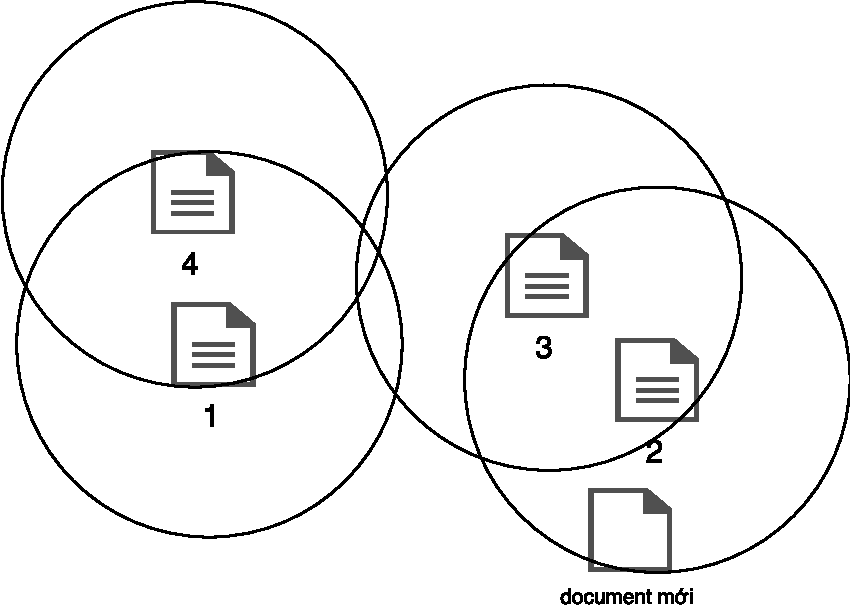
\includegraphics[width=0.9\linewidth]{NNS.pdf}
				\caption{Cách xử lý một document mới trong thuật toán Nearest Neighbor Search}
			\end{center}
		\end{figure}
		
	\subsubsection{Mã giả}
		\begin{algorithm}[H]
			\caption{Phát hiện tin nóng dựa trên k-Nearest neighbor}
			\begin{algorithmic}[1]
				\REQUIRE luồng bài viết từ Twitter, giá trị ngưỡng MergeThreshold
				\ENSURE các cụm bài viết
				\ForEach{document $d$ trong toàn bộ dữ liệu}
					\State $S(d) \leftarrow \emptyset$
					\ForEach{term $t$ trong document $d$}
						\ForEach{document $d'$ trong $index[t]$}
							\State cập nhật độ tương đồng $similarity(d,d')$
							\State $S(d) \leftarrow S(d) \cup d'$
						\ENDFOR 
						\State $index[t] \leftarrow index[t] \cup d$ (thêm document $d$ vào index của term t)
					\ENDFOR
					\STATE similarity score của d: $similarity_{max}(d) \leftarrow 0$
					
					\ForEach{document $d'$ trong S(d)}
						\IF{$similarity(d,d') > similarity_{max}(d)$}
							\STATE $similarity_{max}(d) \leftarrow similarity(d,d')$
						\ENDIF
					\ENDFOR
					\IF{$similarity_{max}(d) < MergeTheshold$}
						\STATE d là một first story
					\ELSE
					
					\ENDIF
				\ENDFOR	
				
			\end{algorithmic}
		\end{algorithm}
		Chú thích thuật toán:
		\begin{itemize}
			\item $MergeThreshold$: ngưỡng để xét một document có phải là first story hay không
			\item $S(d)$: tập document có ít nhất 1 term chung với $d$
			\item $similarity(d,d')$: độ tương đồng giữa document $d$ và $d'$, có thể sử dụng các độ đo ở mục \ref{distances}
			\item $index(t)$: danh sách cách document có chứa term $t$
			\item $dis_{min}(d)$: khoảng cách giữa document $d$ với document gần nhất
		\end{itemize}
		
	\subsubsection{Ưu điểm, hạn chế}
		Ưu điểm:
		\begin{itemize}
			\item Đơn giản và dễ cài đặt.
			\item Có thể chọn nhiều độ đo khoảng cách khác nhau.
			\item Thích nghi tốt với nhiều loại dữ liệu.
		\end{itemize}
		Nhược điểm:
		\begin{itemize}
			\item Chi phí tính toán cao do phải lưu trữ và tính toán trên toàn bộ dữ liệu, không thể áp dụng cho luồng dữ liệu không liên tục.
			\item Độ chính xác giảm khi số chiều của dữ liệu tăng cao.
		\end{itemize}
%========================================================================================================================
	
\subsection{Thuật toán gom cụm có Boost trọng số cho Named Entity}
	\subsubsection{Ý tưởng}
	Cách tiếp cận được đề xuất bởi Phuvipadawat là gom cụm các bài viết theo độ tương tự nội dung, với điểm nhấn là tăng giá trị tương đồng của các bài viết nếu chúng cùng đề cập đến một thực thể có tên (Named entity) nào đó \cite{SwitPhuvipadawat}. Mỗi cụm thu được sẽ ứng với một sự kiện phát hiện được, với document cũ nhất làm đại diện cho cụm đó.
	
	Theo Phuvipadawat, một đặc điểm của các bài viết trên Twitter là thường có nội dung khá ngắn (tối đa 140 kí tự, và ngắn hơn nữa sau khi tiền xử lý loại bỏ stop words). Việc sử dụng phương pháp TF-IDF truyền thống để tính độ tương đồng có thể không đạt được kết quả tốt do không có nhiều term để tìm ra sự tương đồng giữa các document. Vì thế tác giả đã đưa ra phương pháp tăng trọng số cho các danh từ riêng (Named Entity), qua đó tăng độ tương đồng giữa những bài viết cùng thảo luận về một sự vật, sự việc cụ thể nào đó.
		
	Khi một document $d$ mới được đưa vào hệ thống, ta so sánh độ tương đồng giữa $d$ với tất cả cụm hiện có thông qua document đầu tiên trong cụm. Ta chọn ra cụm có độ tương đồng với $d$ cao nhất, gán $d$ vào cụm đó nếu độ tương đồng vượt ngưỡng định trước, ngược lại ta tạo cụm mới với $d$ là document đầu tiên của cụm.
	
	\subsubsection{Minh họa thuật toán}
	Giả sử ta có một số document đã được gom nhóm sẵn thành 3 cụm như hình, ngưỡng MergeThreshold = 0.7, mỗi cụm có một firstDoc làm đại diện. Đường tròn thể hiện ngưỡng khoảng cách để một document được xem là first story hay không.\\
	
	Khi một document mới (newDoc) vào hệ thống: 
	\begin{itemize}
		\item Bước 1: So sánh newDoc với từng firstDoc của từng cụm:\\ 
		$similarity(newDoc, g1.firstDoc) = 0.6$\\
		$similarity(newDoc, g2.firstDoc) = 0.5$\\
		$similarity(newDoc, g3.firstDoc) = 0.35$%Tính ra độ tương đồng
		\item Bước 2: Tìm cụm có firstDoc tương tự với newDoc nhất: Chọn được cụm $g1$%chọn rõ g1...
		\item Bước 3: $similarity(newDoc, g1.firstDoc) = 0.6$ nhỏ hơn MergeThreshold: Tạo cụm g4 với $g4.firstDoc = newDoc$.
	\end{itemize}
	
	%Cho số cụ thể?? 
	\begin{figure}[ht]
		\begin{center}
			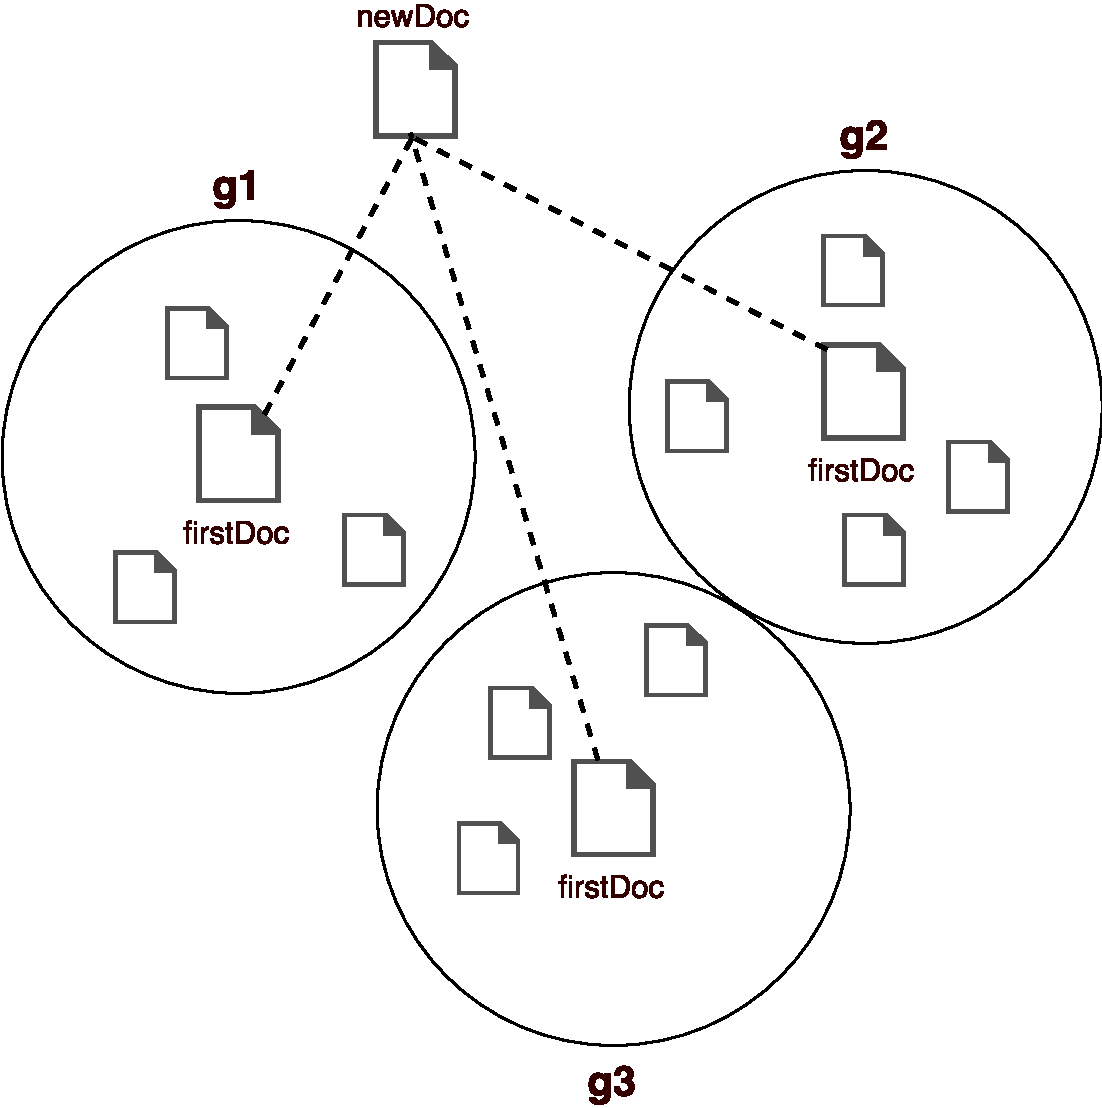
\includegraphics[width=0.65\textwidth]{Clustering_NER2.pdf}
			\caption{Cách xử lý một document mới theo thuật toán Boost Named Entity}
		\end{center}
	\end{figure}
	
	\subsubsection{Mã giả}
	\begin{algorithm}[H]
		\caption{Phát hiện tin nóng sử dụng gom cụm theo nội dung, boost Named Entity}
		\begin{algorithmic}[1]
			\REQUIRE luồng bài viết từ Twitter, giá trị ngưỡng MergeThreshold
			\ENSURE các cụm bài viết ứng với mỗi story phát hiện được, có thứ tự xếp hạng giữa các cụm

			\ForEach{document $d$ trong toàn bộ dữ liệu}
				\State $MaxScore_d \leftarrow 0$
				\State $IDMaxScore_d \leftarrow \emptyset$
				\ForEach{cụm g trong tập hợp cụm G}
%					\State tính $Score_d[g]$: độ tương đồng giữa $d$ với $g.firstDoc$, chỉ dùng một số topTerms của $g$
					\State tính $Score_d[g] \leftarrow similarity(d, g.firstDoc)$
					
					\IF{$MaxScore_d < Score_d[g]$}
						\State $MaxScore_d \leftarrow Score_d[g]$
						\State $IDMaxScore_d \leftarrow g.groupID$
					\ENDIF
				\ENDFOR
				
				\IF{$MaxScore_d$ > MergeThreshold}
					\State gán $d$ vào cụm $IDMaxScore_d$
				\ELSE
					\State tạo cụm $g_{new}$
					\State $g_{new}.firstDoc \leftarrow d$
				\ENDIF
			\ENDFOR
		\end{algorithmic}
	\end{algorithm}
	Chú thích thuật toán:
	\begin{itemize}
		\item $MaxScore_d$: chứa độ tương đồng lớn nhất giữa document d và các cụm đã có
		\item $IDMaxScore_d$: ID của cụm tương đồng nhất với document d
		\item $Score_d[g]$: độ tương đồng giữa document d với cụm g 
		\item $MergeThreshold$: ngưỡng để xét một document có thuộc về cụm/có là first story hay không
	\end{itemize}
	Độ tương đồng giữa 2 document được tính bằng các công thức sau:
	\begin{equation}
			similarity(d_1, d_2) = \sum_{t \in d_1,\ t \in g.topTerms}[tf(t, d_2) \times idf(t) \times boost(t)]
	\end{equation}
	\begin{equation}
		tf(t, d) = \frac{count(t \in d)}{size(d)}
	\end{equation}
	\begin{equation}
		idf(t) = 1 + \log\frac{N}{count(m\ has\ t)}
	\end{equation}
	Các kí hiệu: 
	\begin{itemize}
		\item $similarity(d_1, d_2)$: độ tương đồng giữa document $d_1$ và document $d_2$
		\item $boost(t)$: giá trị boost cho term t, nếu t là một danh từ riêng (Named Entity) thì boost(t) > 1, ngược lại boost(t) = 1
		\item $tf(t, d)$: tần suất xuất hiện (theo phần trăm) của term t trong document d
		\item $count(t \in d)$: tần suất term t xuất hiện trong trong document d
		\item $size(d)$: số lượng term của document d
		\item $idf(t)$: giá trị inverse document frequency của term t
		\item $N$: tổng số document trong hệ thống
		\item $count(m\ has\ t)$: số document có chứa term t
	\end{itemize}

	\subsubsection{Ưu điểm, hạn chế}
	Ưu điểm:
	\begin{itemize}
		\item Dễ gom nhóm được các sự kiện bàn về cùng thực thể nào đó.
	\end{itemize}
	Nhược điểm:
	\begin{itemize}
		\item Chất lượng kết quả gom cụm phụ thuộc một phần vào việc phát hiện được thực thể có tên.
	\end{itemize}

%========================================================================================================================
\subsection{Thuật toán Locality Sensitive Hashing}
	\subsubsection{Ý tưởng}
%	(O(nd) với n là số lượng document hiện có và d là số chiều của mỗi document)
	Thuật toán tìm kiếm láng giềng gần nhất tốn rất nhiều chi phí khi lượng dữ càng lớn. Thay vào đó, ta có thể giải bài toán tìm \textit{xấp xỉ} láng giềng gần nhất. Một thuật toán để giải quyết bài toán này là \textit{Locality Sensitive Hashing (LSH)} được đề xuất bởi Piotr Indyk và cộng sự \cite{Indyk:LSH-Definition}.
	
	LSH hoạt động bằng cách chia không gian biểu diễn dữ liệu thành nhiều vùng riêng biệt bằng một tập các siêu phẳng ngẫu nhiên. Ta có thể xem mỗi cách chia không gian này ứng với một hash table, và số bit của hash code bằng với số lượng siêu phẳng đã dùng để chia không gian. Mỗi khi một document mới vào hệ thống, ta tính hash code của nó. Khi cần tìm láng giềng cho một document, ta chỉ cần so sánh nó với các document thuộc chung vùng không gian (ứng với một bucket trong hash table), nhờ đó giảm đáng kể chi phí tính toán.
	
%	Ta có thể thấy khi tăng số lượng siêu phẳng lên thì số lượng document rơi vào cùng một vùng không gian sẽ càng giảm, do kích cỡ của vùng không gian nhỏ, th
	
	Vì các siêu phẳng được chọn một cách ngẫu nhiên, nên đôi khi các document dù gần nhau vẫn có thể bị phân vào vùng khác nhau. Do đó ta thường dùng cùng lúc nhiều hash table để tăng thêm khả năng tìm được láng giềng gần nhất.	
%	LSH sử dụng một họ hash function (hàm băm) có đặc điểm: những documents càng tương đồng với nhau thì càng có khả năng trùng hash code (mã băm) với nhau. Mỗi document mới sẽ được đưa qua hash function tính toán, và sau đó được so sánh với các document có cùng hash code với nó.\\

	\subsubsection{Minh họa cách tính hash code cho LSH}
%	Xét trường hợp một document $d$ biểu diễn dưới dạng vector $d = (0,1,0,1,1,1,0)$, và ta chọn sử dụng hash code có 4 bit (dùng 4 siêu phẳng để chia không gian dữ liệu).\\
%	Mỗi hash table được khởi tạo bằng cách: tạo 4 vector ngẫu nhiên ứng với 4 siêu phẳng, số chiều bằng với số chiều vector $d$
%	Cách tính hash code của document $d$ trong một hash table như sau: lần lượt tính tích vô hướng của vector $d$ với từng vector của siêu phẳng, nếu tích dương thì bit đó có giá trị 1, nếu tích âm thì có giá trị 0. 
		
	Giả sử ta có không gian biểu diễn document gồm 7 từ/term khác nhau (8 chiều). Xét một document $d$ biểu diễn dưới dạng vector $d = (0,1,0,1,1,1,0)$, và ta chọn sử dụng hash code có 4 bit (dùng 4 siêu phẳng để chia không gian dữ liệu).
	
	Mỗi hash table được khởi tạo bằng cách: tạo 4 vector ngẫu nhiên ứng với 4 siêu phẳng, số chiều bằng 7, ứng với số chiều của vector $d$.
	
	Cách tính hash code của document $d$ trong một hash table như sau: lần lượt tính tích vô hướng của vector $d$ với từng vector của các siêu phẳng, nếu tích dương thì bit đó có giá trị 1, nếu tích âm thì có giá trị 0. 
	
	\begin{figure}[ht]
		\begin{center}
			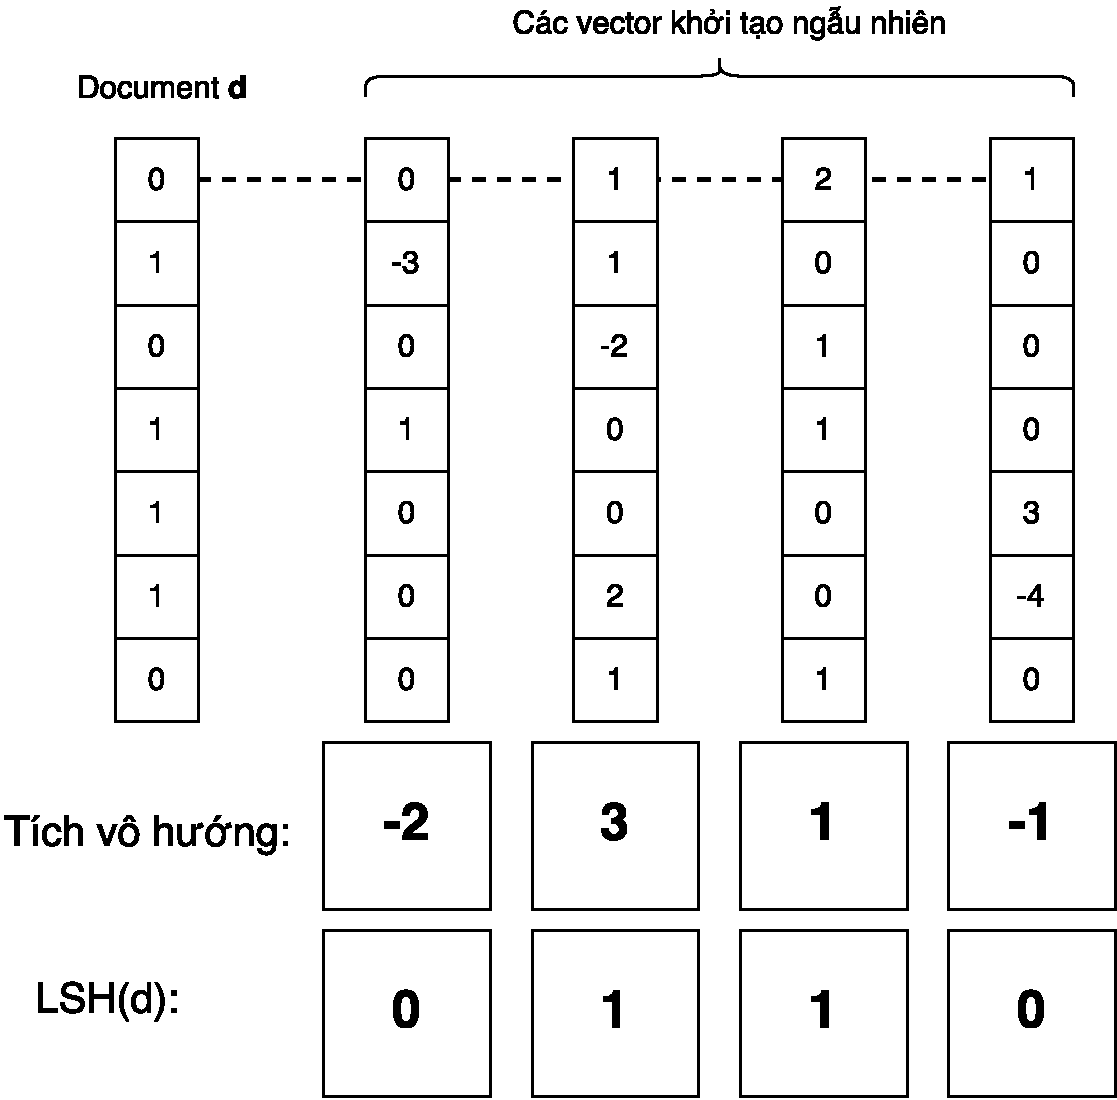
\includegraphics[width=0.65\textwidth]{LSH.pdf}
			\caption{Cách tính hash code cho một document trong một hash table}
		\end{center}
	\end{figure}
	
	\subsubsection{Mã giả}
	\begin{algorithm}[H]
		\caption{Phát hiện tin nóng sử dụng Locality Sensitive Hashing}
		\begin{algorithmic}[1]
			\REQUIRE luồng bài viết từ Twitter, giá trị ngưỡng t
			\ENSURE những cụm bài viết
			\State Khởi tạo L hash tables
			\ForEach{document $d$ mới}
				\ForEach{hash table $l$ trong $L$}
					\State Tính hash code cho document d: $LSH_l(d)$
					\State Thêm tất cả các documents d' có $LSH_l(d') = LSH_l(d)$ vào tập $S$
				\ENDFOR
				\State $dis_{min}(d) = 1$
				\ForEach{document $d'$ trong $S$}
					\IF {$distance(d,d') < dis_{min}(d)$}
					\STATE $dis_{min}(d) = distance(d,d')$
		 			\ENDIF
				\ENDFOR
				\IF{$dis_{min}(d) >= t$}
					\STATE tạo cụm mới chứa d
				\ELSE
					\STATE thêm d vào cụm chứa hàng xóm gần nhất của d
				\ENDIF
			\ENDFOR
			
		\end{algorithmic}
	\end{algorithm}
	Chú thích thuật toán:
	\begin{itemize}
		\item $t$: ngưỡng để xét một document có phải là first story hay không
		\item $LSH_l(d)$: hash code của document $d$ trong hash table thứ $l$
		\item $dis_{min}(d)$: khoảng cách giữa document $d$ với document gần nhất
		
	\end{itemize}
	
	Ưu điểm:
	\begin{itemize}
		\item Chi phí tính toán thấp do không cần so sánh toàn bộ các document với nhau.
		\item Độ chính xác tương đối tốt
	\end{itemize}

	Nhược điểm:
	\begin{itemize}
		\item Cần tìm chọn các thông số như: số lượng hash table, số lượng bit trong hash code,... tốt để cho kết quả chính xác.
		\item Có thể không tìm được document thật sự tương đồng nhất, trong trường hợp các điểm không được chia vào cùng vùng trong không gian do cách thiết lập của các siêu phẳng trong hash tables.
	\end{itemize}
	
	\subsubsection{LSH cải tiến}
	Dựa vào dữ liệu thực nghiệm của mình, Sasa Petrovic và cộng sự \cite{Petrovic:LSH} đưa ra nhận định rằng việc áp dụng LSH thuần túy vào bài toán FSD cho ra kết quả chưa tốt. Trong trường hợp điểm dữ liệu cách xa tất cả điểm còn lại, LSH không tìm được láng giềng gần nhất, do không có điểm nào khác rơi vào cùng bucket trong các hash table, dẫn đến không có điểm dữ liệu khác để so sánh. 
	
	Để giải quyết vấn đề này, Petrovic đưa ra phương án: mỗi khi tìm ra document $d$ có $dis_{min}(d)$ lớn hơn ngưỡng, ta áp dụng thuật toán tìm láng giềng gần nhất giữa document $d$ và khoảng 1000 tới 3000 document có thời gian gần đây nhất trong hệ thống, cập nhật giá trị $dis_{min}(d)$ và xét xem nó vẫn vượt ngưỡng hay không, nếu có thì ta kết luận $d$ là một first story, ngược lại ta cho $d$ vào cụm của láng giềng gần nó nhất.
	
	\begin{algorithm}[H]
		\caption{Phát hiện tin nóng sử dụng Locality Sensitive Hashing kết hợp với Nearest Neighbor Search}
		\begin{algorithmic}[1]
%			\boldmath
			\REQUIRE luồng bài viết từ Twitter, giá trị ngưỡng t
			\ENSURE những cum bài viết
			\State Khởi tạo L hash tables
			\ForEach{document $d$ mới}
				\ForEach{hash table $l$ trong $L$}
					\State Tính hash code cho document d: $LSH_l(d)$
					\State Thêm tất cả các documents d' có $LSH_l(d') = LSH_l(d)$ vào tập $S$
				\ENDFOR
				\State $dis_{min}(d) = 1$
				\ForEach{document $d'$ trong $S$}
					\unboldmath
					\IF {$distance(d,d') < dis_{min}(d)$}
					\State $dis_{min}(d) = distance(d,d')$
					\ENDIF
				\ENDFOR
				\IF{$dis_{min}(d) >= t$}
					\State Tính khoảng cách giữa d với một lượng (1000-3000) documents mới nhất trong bộ dữ liệu, cập nhật $dis_{min}(d)$ nếu có thay đổi.
				\ENDIF
				\IF{$dis_{min}(d) >= t$}
					\STATE tạo cụm mới chứa d
				\ELSE
					\STATE thêm d vào cụm chứa hàng xóm gần nhất của d
				\ENDIF
			\ENDFOR		
			
		\end{algorithmic}
	\end{algorithm}

\section{Giới thiệu một số độ đo đánh giá phân lớp} \label{clusterEvalMetrics}
Đánh giá chất lượng của kết quả gom cụm là nhiệm vụ khó khăn và phức tạp, do bản chất không hoàn toàn rõ ràng về định nghĩa của một "cụm". Theo tác giả Pang-Ning Tan và cộng sự \cite{IntroToDM}, có 3 loại phương pháp để đánh giá chất lượng cụm: 
	\begin{itemize}
		\item Đánh giá ngoại, có giám sát (External evaluation): Các độ đo có sử dụng thông tin bên ngoài như nhãn lớp của dữ liệu để so sánh với kết quả gom cụm.
		VD: Purity, Rand measure,...
		\item Đánh giá nội, không giám sát (Internal evaluation): Chỉ dựa vào các thông tin, thuộc tính có sẵn trong cụm để đánh giá.
		VD: Silhouette index, Dunn index, Davies–Bouldin index...
		\item Đánh giá tương đối (Relative evaluation): So sánh kết quả giữa các phương pháp gom cụm hoặc giữa các cụm, có thể dùng độ đo ngoại lẫn nội.
	\end{itemize}

%Khóa luận này chỉ xem xét đến các chỉ số đánh giá nội, do hạn chế về mặt dữ liệu tin tức có gán nhãn lớp.
	\subsection{Khoảng cách cục bộ và toàn cục (Intra-cluster và Inter-cluster distance)} \label{localglobaldistance}
	Hai độ đo này thuộc loại đánh giá nội, chỉ dựa vào chính dữ liệu được gom cụm để tính giá trị của chúng. Khoảng cách cục bộ của một cụm thể hiện mức độ các điểm dữ liệu trong một cụm tương đồng với nhau thế nào. Dưới đây là 3 cách để tính khoảng cách cục bộ:
		\begin{itemize}
			\item Dùng khoảng cách giữa 2 điểm xa nhau nhất trong cụm:\\
			\scalebox{1.1}{$intraclusterDistance(C_i) = \ max_{x, y \in C_i} distance(x, y)$}
			
			\item Dùng trung bình khoảng cách giữa tất cả cặp điểm trong cụm:\\
			\scalebox{1.1}{$intraclusterDistance(C_i) = \frac{1}{size(C_i) \ *\ [size(C_i)-1]} \sum_{x, y \in C_i, x \ne y} distance(x, y)$ }\\
			
			\item Dùng trung bình khoảng cách giữa từng điểm với tâm cụm:\\
			\scalebox{1.1}{$intraclusterDistance(C_i) = \frac{\sum_{x \in C_i} distance(x, \mu)}{size(C_i)} $, $\mu = \frac{\sum_{x \in C_i} x}{size(C_i)}$}\\	
		\end{itemize}
	
	Khoảng cách toàn cục là giá trị cho thấy mức độ rời rạc giữa tất cả các cụm với nhau, được tính bằng trung bình khoảng cách giữa các cụm:
		\begin{equation}
			interclusterDistance = \frac{1}{size(C) * [size(C)-1]} \sum_{C_i, C_j \in C} distance(C_i, C_j)
		\end{equation}
	
	Trong đó, khoảng cách giữa 2 cụm $distance(C_i, C_j)$ cũng có thế được xác định bằng nhiều cách như:
		\begin{itemize}
			\item Dùng khoảng cách giữa 2 điểm xa nhau nhất trong 2 cụm:\\
			\scalebox{1.1}{$distance(C_i, C_j) = \ max_{x \in C_i, y \in C_j} distance(x, y)$}
			
			\item Dùng trung bình khoảng cách giữa tất cả cặp điểm trong 2 cụm:\\
			\scalebox{1.1}{$distance(C_i, C_j) = \frac{1}{size(C_i) + size(C_j)} \sum_{x \in C_i, y \in C_j} distance(x, y)$ }
			
			\item Dùng khoảng cách giữa 2 tâm cụm:\\
			\scalebox{1.1}{$distance(C_i, C_j) = distance(\mu_{C_i}, \mu_{C_j})$, với $\mu_{C_i} = \frac{\sum_{x \in C_i} x}{size(C_i)}$}
%			\scalebox{1.1}{$\mu_{C_i} = \frac{\sum_{x \in C_i} distance(x, \mu)}{size(C_i)}$}\\	
	\end{itemize}

	Chú thích kí hiệu: 
	\begin{itemize}
		\item $C_i$: cụm dữ liệu thứ $i$
%		\item $localDistance(C_i)$: khoảng cách cục bộ của cụm $i$
		\item $x, y$: 2 điểm dữ liệu bất kì
		\item $distance(x, y)$: khoảng cách giữa 2 điểm dữ liệu, dùng các khoảng cách ở mục \ref{distances}
		\item $size(C_i)$: số lượng điểm dữ liệu được gom vào cụm $i$
	\end{itemize}
	\subsection{Độ đo Dunn index}
	Dunn index được đề xuất bởi J. C. Dunn \cite{dunn1973fuzzy2}, độ đo này thể hiện mức độ gắn kết của từng cụm lẫn độ rời rạc giữa các cụm. Giá trị Dunn index được tính theo công thức sau:	
		\begin{equation} \label{dunnindex}
		DI = \frac{min_{1 \leq i \leq j \leq n}distance(C_i, C_j)}{max_{1 \leq k \leq n}intraclusterDistance(k)}
		\end{equation}
		
		Với $n$ là tổng số cụm thu được, và intraclusterDistance được tính theo một trong những cách ở mục \ref{localglobaldistance}.
		
	Giá trị Dunn index càng cao thì các cụm càng tách biệt nhau và mỗi cụm thì có những điểm dữ liệu gom sát với nhau. Tuy vậy, mẫu số trong công thức (\ref{dunnindex}) lấy khoảng cách cục bộ của cụm rời rạc nhất chứ không lấy trung bình tất cả cụm, nên giá trị Dunn index là trường hợp xấu nhất chứ không phải trường hợp trung bình.
	\subsection{Hệ số Silhouette (Silhouette coefficient)}
%	Cohesion và separation
	
	Silhouette là một độ đo xem xét các đối tượng trong dữ liệu có được gán vào cụm hợp lý hay không, thông qua việc so sánh cả độ gắn kết của từng cụm và độ rời rạc giữa các cụm. Với mỗi điểm dữ liệu, giá trị silhouette coefficient nằm trong khoảng từ -1 đến 1, giá trị này cao khi điểm dữ liệu tương đồng với cụm của nó và ít tương đồng với cụm khác, và ngược lại. 
	
	Cách tính hệ số Silhouette cho một điểm dữ liệu \textbf{i} như sau:
	\begin{enumerate}
		\item Tính khoảng cách trung bình giữa i với các điểm trong cùng cụm với i. Gọi giá trị này là $a_i$.
		\item Với mỗi cụm g không chứa i, tính khoảng cách của i đến cụm g bằng trung bình khoảng cách giữa i với từng điểm trong cụm g, chọn cụm có khoảng cách đến i \textit{nhỏ nhất}. Gọi giá trị này là $b_i$
		\item Tính hệ số Silhouette theo công thức sau:
		\begin{equation}
		s(i) = \frac{b_i - a_i}{max\{a_i,b_i\}}
		\end{equation}
	\end{enumerate}
	
	Ở đây $a_i$ đại diện cho độ bất phù hợp của điểm i với cụm của nó, và $b_i$ đại diện cho độ tương đồng giữa điểm i với cụm gần nhất không chứa i. Vì vậy khi $a_i$ nhỏ, $b_i$ lớn, giá trị hệ số silhouette tiến tới 1, nghĩa là điểm dữ liệu i rất phù hợp với cụm của nó và không phù hợp với cụm khác. Trong trường hợp ngược lại, giá trị silhouette tiến tới -1.
	
	Giá trị hệ số Silhouette cho một kết quả phân cụm được tính bằng trung bình hệ số Silhouette của tất cả điểm dữ liệu.

	\subsection{Độ đo Purity}
	Đây là một độ đo đánh giá ngoại. Dựa trên nhãn lớp của dữ liệu, purity là độ đo về tính thuần khiết/độ đồng nhất của các cụm. Giá trị này tính bằng cách lấy tần số của lớp chiếm số lượng nhiều nhất trong cụm (tính theo phần trăm kích cỡ cụm). Purity càng cao khi cụm chứa càng nhiều điểm dữ liệu thuộc cùng một nhãn lớp.\\
	
	Giá trị purity của một cụm $C_i$ được tính bằng công thức:
	\begin{equation}
	purity(C_i) = max_j( \frac{m_{ij}}{m_i})
	\end{equation}
	
	Trong đó:
	\begin{itemize}
		\item $m_i$: số điểm dữ liệu thuộc cụm i
		\item $m_{ij}$: số điểm dữ liệu thuộc lớp j và nằm trong cụm i
	\end{itemize}
	
	Giá trị purity của tất cả cụm được tính như sau:
	\begin{equation}
	purity = \sum_{i=1}^{K} \frac{m_i}{m} \ purity(C_i)
	\end{equation}
	
	Trong đó:
	\begin{itemize}
		\item $K$: tổng số cụm
		\item $m$: tổng số điểm dữ liệu
	\end{itemize}
	
\section{Xếp hạng cụm}
	Một yêu cầu của bài toán phát hiện tin nóng là các chuỗi tin (ứng với các cụm) phải được sắp xếp theo mức độ nóng giảm dần. Hầu hết các phương pháp đã khảo sát trong khóa luận này chỉ tập trung vào việc gom cụm và cải thiện chất lượng cụm, mà không đề cập đến việc sắp xếp cụm theo thứ tự nào đó. 
	
	Tác giả Phuvipadawat đưa ra một số công thức để tính điểm lượng giá độ nóng của chuỗi tin, và các chuỗi tin được sắp xếp theo giá trị điểm giảm dần \cite{SwitPhuvipadawat}.
	
%	Các cụm được xếp hạng bằng công thức được đề xuất bởi Phuvipadawat \cite{SwitPhuvipadawat}, mỗi cụm được gán một giá trị điểm, và dùng điểm đó để so sánh giữa các cụm, cụm có điểm cao nhất sẽ được sắp xếp lên đầu.
	
	Điểm này cân nhắc tầm ảnh hưởng của những người viết bài trong cụm, cũng như mức độ lan tỏa của chính các bài viết trong cụm. Giá trị điểm cũng được cập nhật thường xuyên và sẽ giảm dần theo thời gian nếu không có những bài viết mới làm tăng điểm cho nó. So với công thức của Phuvipadawat, công thức 2.12 bổ sung thêm yếu tố lượng favorite của cụm, do đây cũng là một thành phần ghi nhận phản ứng từ người dùng Twitter.
	
	Giá trị điểm xếp hạng của một cụm $C_i$ được cho bằng công thức sau:
	\begin{equation}
		Score(C_i) = \frac{1}{Z} \sum_{j = 1}^k \frac{S_i}{log_2(\Delta_j + 2)}
	\end{equation}
	
	Với $S_i$ tính bằng:
	\begin{multline}
	S_i = w_1 \sum_{u_i \in C_i} FollowerCount(u_i) + w_2\ TotalRetweetCount(C_i)\\ + w_3\ TotalFavoriteCount(C_i)
	\end{multline}

	Trong đó:
	\begin{itemize}
		\item $\frac{1}{Z}$: giá trị để chuẩn hóa điểm cụm, Z là tổng điểm của các cụm khi chưa chuẩn hóa
		\item $k$: số lượng document trong cụm
		\item $\Delta_j$: chênh lệch thời gian giữa thời điểm hiện tại với thời gian bài viết $j$ được đăng
		\item $w_1, w_2$: trọng số cho hai vế của biểu thức
		\item $u_i$: người dùng thứ $i$
		\item $FollowerCount(u_i)$: số người follow người dùng $u_i$ trên Twitter
		\item $TotalRetweetCount(g_i)$: tổng số retweet của các bài đăng trong cụm $c_i$
	\end{itemize}
\section{Kết chương}
Chương này đã phát biểu bài toán phát hiện tin nóng và đưa ra 4 thuật toán tiếp cận theo hướng gom cụm. Đồng thời trình bày về các độ đo tương đồng, độ đo đánh giá chất lượng cụm và cách xếp hạng cụm. Chương tiếp theo sẽ trình bày về việc xây dựng hệ thống phát hiện tin nóng.